\documentclass[11pt]{article}
\usepackage[utf8]{inputenc}
\usepackage[T1]{fontenc}
\usepackage[french]{babel}
\usepackage{fullpage}
\usepackage{microtype}

\usepackage{amsthm}
\usepackage{amsmath}
\usepackage{amssymb}
\usepackage{stmaryrd}
\usepackage{enumitem}
\usepackage{siunitx}
\usepackage{graphicx}
\usepackage{minted}
\usepackage{subcaption}
\usepackage{hyperref}

\DeclareMathOperator{\e}{e}
\DeclareMathOperator{\Id}{Id}
\DeclareMathOperator{\Idm}{I}
\DeclareMathOperator{\Ker}{Ker}
\DeclareMathOperator{\Ima}{Im}
\DeclareMathOperator{\Vect}{Vect}
\DeclareMathOperator{\rg}{rg}
\DeclareMathOperator{\GL}{GL}
\DeclareMathOperator{\tr}{tr}
\DeclareMathOperator{\Com}{Com}
\DeclareMathOperator{\Sp}{Sp}

\newcommand{\ensemble}[1]{\mathbb{#1}}
\newcommand{\N}{\ensemble{N}}
\newcommand{\Z}{\ensemble{Z}}
\newcommand{\Q}{\ensemble{Q}}
\newcommand{\R}{\ensemble{R}}
\newcommand{\C}{\ensemble{C}}
\newcommand{\K}{\ensemble{K}}

\newcommand{\notation}[1]{\mathcal{#1}}
\newcommand{\classeC}{\notation{C}}
\newcommand{\mat}{\notation{M}}
\newcommand{\edm}{\notation{L}}
\newcommand{\ortg}{\notation{O}}
\newcommand{\sym}{\notation{S}}

\newcommand{\intervalle}[4]{\mathopen{#1}#2 \mathclose{}\mathpunct{},#3 \mathclose{#4}}
\newcommand{\intff}[2]{\intervalle{[}{#1}{#2}{]}}
\newcommand{\intof}[2]{\intervalle{]}{#1}{#2}{]}}
\newcommand{\intfo}[2]{\intervalle{[}{#1}{#2}{[}}
\newcommand{\intoo}[2]{\intervalle{]}{#1}{#2}{[}}
\newcommand{\intent}[2]{\intervalle\llbracket{#1}{#2}\rrbracket}

\newcommand{\diff}{\mathop{}\mathopen{}\mathrm{d}}
\newcommand{\norme}[1]{\left\lVert#1\right\rVert}
\newcommand{\petito}[1]{o\mathopen{}\left(#1\right)}
\newcommand{\grandO}[1]{O\mathopen{}\left(#1\right)}
\newcommand{\enstq}[2]{\left\{#1\mathrel{}\middle|\mathrel{}#2\right\}}
\newcommand{\prodscal}[2]{\left\langle#1,#2\right\rangle}
\newcommand{\restreinta}{\mathclose{}|\mathopen{}}
\newcommand{\integrale}[2]{\displaystyle \int_{#1}^{#2}}
\newcommand{\somme}[2]{\sum\limits_{#1}^{#2}}
\newcommand{\produit}[2]{\prod\limits_{#1}^{#2}}
\newcommand{\derp}[2][]{\frac{\partial#1}{\partial#2}}

\newcommand{\fonction}[5]
{\begin{array}{lrcl}
#1 : & #2 & \longrightarrow & #3 \\
     & #4 & \longmapsto & #5 \end{array}}
     
\newcommand{\ie}{\textsl{i.e.}\ }

\title{Étude et modélisation d'un système proie-prédateur par un automate cellulaire}
\author{Olivier \bsc{Roques}}
\date{2015-2016}

\begin{document}

\maketitle

\renewcommand{\contentsname}{Sommaire}
\tableofcontents
\newpage

\section{Introduction}

La dynamique des populations est une branche des mathématiques et de l'écologie qui s'intéresse aux variations de la population d'une espèce, en tenant compte de l'influence du milieu et des interactions inter-espèces. De nos jours, avec la prise de conscience collective de la fragilité des écosystèmes, ce domaine des sciences est devenu essentiel dans la lutte pour la préservation de la faune et de la flore.

Mon étude se limite ici à un écosystème constitué de deux espèces, l'une faisant office de proie et l'autre de prédateur. De plus, l'évolution des effectifs est supposée continue dans le temps et déterministe, c'est-à-dire régie par des équations différentielles et par la donnée d'un état initial.

L'objet de cet exposé est de comprendre comment modéliser théoriquement les fluctuations de population d'un couple proie-prédateur, avant d'en proposer une simulation informatique réaliste à travers l'implémentation d'un automate cellulaire graphique sous Python.

J'aborde d'abord les équations proie-prédateur de \bsc{Lotka}-\bsc{Volterra} et le comportement de ses solutions pour les confronter à une évolution réelle de populations. Cette première approche me permet ainsi de poser les fondements d'une adaptation informatique, aboutissant au développement d'un automate cellulaire paramétrable et dynamique simulant le comportement des espèces dans leur habitat. C'est enfin avec ce programme que je me suis intéressé à l'influence du milieu et des variables propres aux espèces sur la dynamique et la stabilité des deux populations.

Dans la suite, $x(t)$ désignera le nombre de proie et $y(t)$ le nombre de prédateurs à l'instant $t$.

\section{Le modèle proie-prédateur de \bsc{Lotka}-\bsc{Volterra}}


\subsection{Énoncé du modèle}

Les travaux d'Alfred \bsc{Lotka} $(1880-1949)$ et Vito \bsc{Volterra} $(1860-1940)$ ont donné naissance en $1925$ à un nouveau champ liant mathématiques et écologie étudiant les évolutions de population d'êtres vivants. Ils présentent indépendamment le même modèle pour décrire les variations de populations, qui s'écrit sous la forme d'un système couplé d'équations différentielles non linéaires du premier ordre selon une variable temporelle $t$:
\[(LK): \begin{cases}
x' = x (\alpha - \beta y )\\
y' = y (- \gamma + \delta x )\\
x(0) = x_0,\ y(0) = y_0
\end{cases}\]

Ce système est donc caractérisé par un nombre initial $x_0$ de proies et $y_0$ de prédateurs et par $4$ paramètres positifs relatifs aux espèces:
\begin{itemize}[label=\textbullet]
    \item $\alpha$ est le taux de reproduction des proies;
    \item $\beta$ est le taux de mortalité des proies face aux prédateurs;
    \item $\gamma$ est le taux de perte des prédateurs (mort naturelle ou émigration);
    \item $\delta$ est le taux de reproduction des prédateurs.
\end{itemize}

\subsection{Étude des solutions}

On peut montrer que les solutions de $(LK)$ sont définie sur $\R$ et périodiques. On observe de plus un état d'équilibre aux points de coordonnées $(0, 0)$ et $\left( \frac{\gamma}{\delta}, \frac{\alpha}{\beta} \right)$. La solution d'un système est présentée figure \ref{fig:solution}.

\begin{figure}[!ht]
    \begin{subfigure}{0.49\textwidth}
        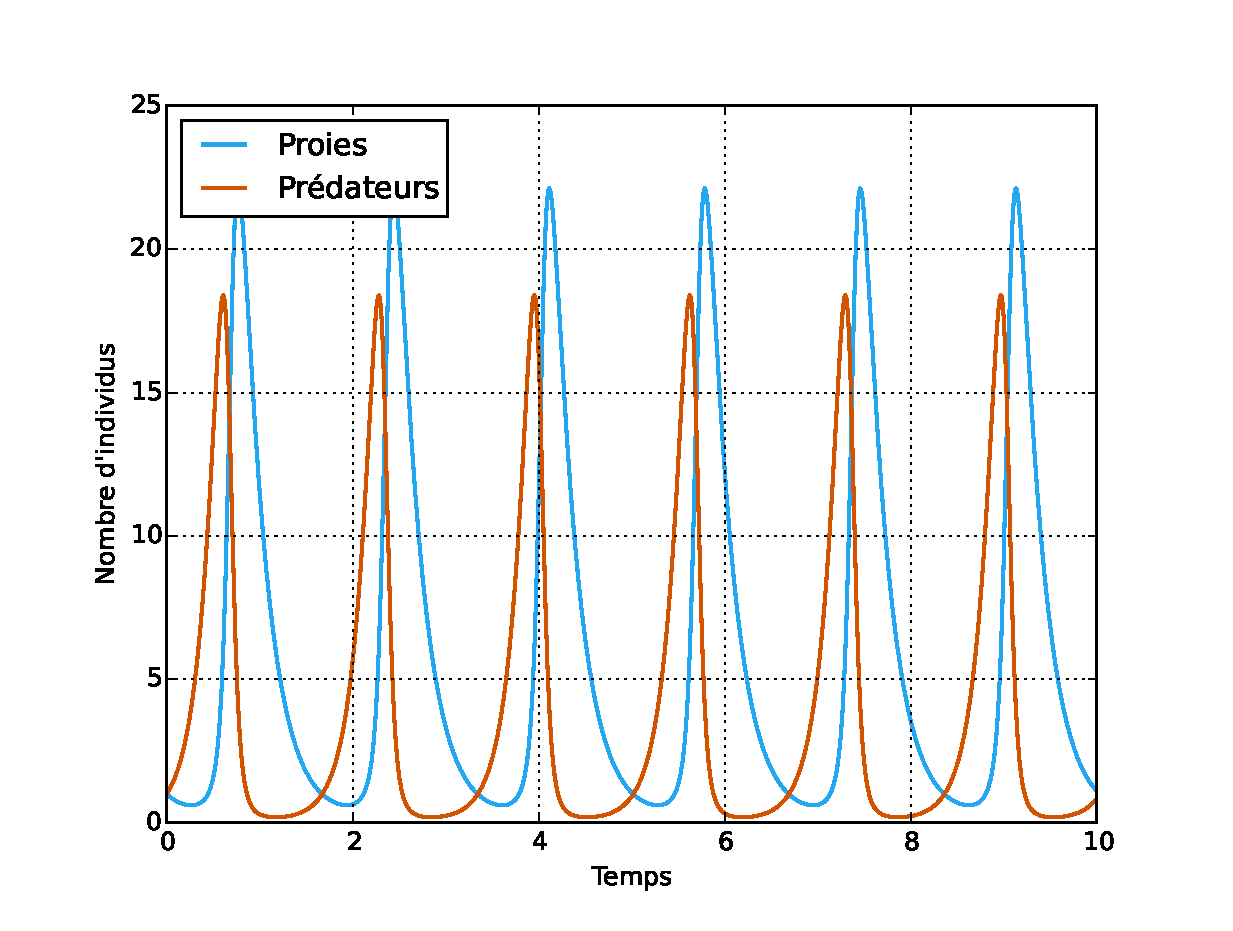
\includegraphics[width=\linewidth]{diagramme_lv.eps} 
        \caption{Graphe obtenu}
    \end{subfigure}
    \begin{subfigure}{0.49\textwidth}
        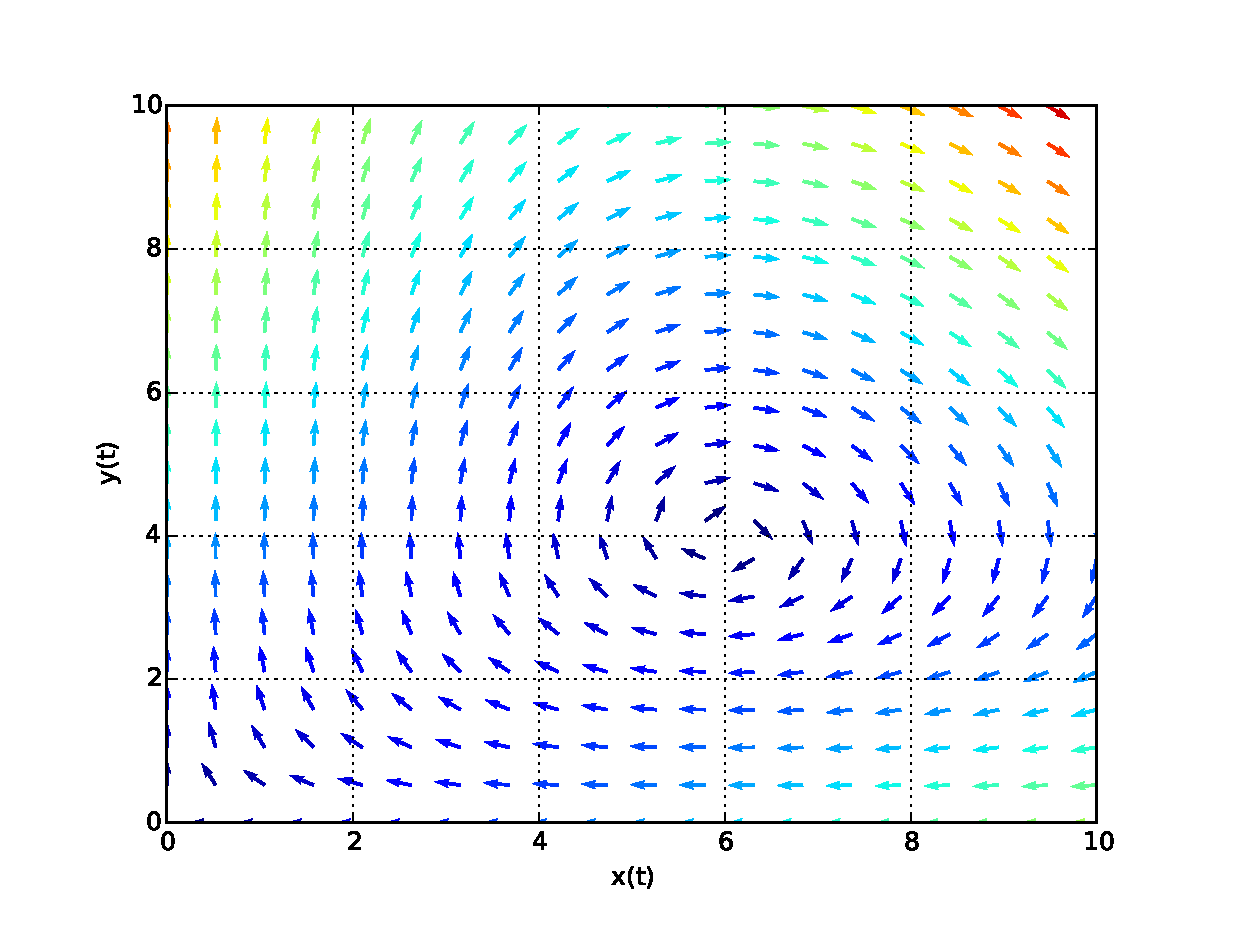
\includegraphics[width=\linewidth]{champ_vecteur.eps}
        \caption{Champ de vecteurs associé}
    \end{subfigure}
     
    \caption{Allure de la solution pour $(x0, y0) = (1, 1)$ et $(\alpha, \beta, \gamma, \delta) = (4, 1, 6, 1)$}
    \label{fig:solution}
\end{figure}

\paragraph{Un exemple d'une évolution de population réelle}
Des relevés réguliers des populations de lièvres et de lynx présents dans la Baie d'Hudson au Canada entre 1845 et 1840 effectués par la Compagnie de la baie d'Hudson donnent une idée de l'évolution réelle d'un couple proie-prédateurs (figure \ref{fig:baie_hudson}).
\begin{figure}[!ht]
    \centering
    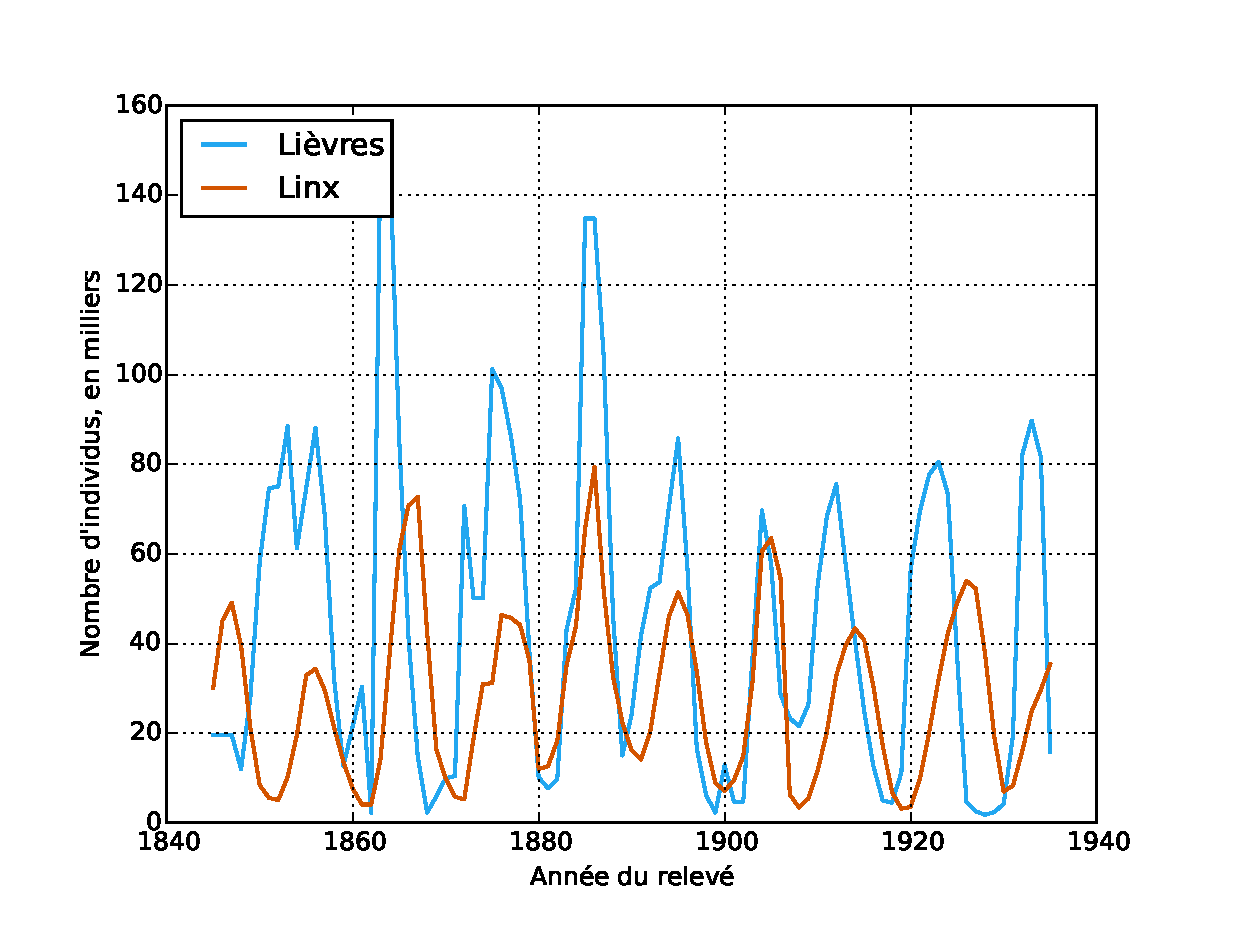
\includegraphics[width=15cm]{evolution.eps}
    \caption{Évolution des populations de lièvres et de lynx de la Baie d'Hudson}
    \label{fig:baie_hudson}
\end{figure}

\subsection{Les limites du modèle}\label{limites}
Ce modèle sommaire présente quelques inconvénients:
\begin{itemize}[label=\textendash]
    \item Il est déjà limité à l'interaction entre deux espèces seulement.
    \item Les ressources limitées du milieu ne sont pas prises en compte: les proies ont ainsi un accès illimité à la nourriture et les événements naturels (saisons, catastrophes) sont ignorés.
    \item Lorsque la population de prédateurs reste nulle, \ie $y(t) = 0\ \forall t$, le modèle prévoit une croissance exponentielle de la population de proies. En effet, on a alors $x'(t) = \alpha x(t)$ qui se résout en $x(t) = x_0\e^{\alpha t}$ et donc qui diverge en l'infini.
    \item Le nombre de prédateurs croît proportionnellement au nombre de proies. En d'autres termes, le modèle suppose l'appétit illimité et instantanément satisfait des prédateurs.  
\end{itemize}

Il existe d'autres modèles, plus complexes, qui tiennent compte des ces contraintes. Par exemple le modèle \emph{Lotka-Volterra avec compétition entre proies} empêche la divergence des proies en l'absence de prédateurs en changeant la première équation ($\alpha$, $\beta$ sont des paramètres positifs):
\[\begin{cases}
x' =x(1-x-y)\\
y' =\beta(x-\alpha)y
\end{cases} \]
\noindent Ou encore le modèle de \bsc{Rosenzweig}-\bsc{MacArthur} dans lequel l'interaction entre proies et prédateurs n'est plus proportionnel à la population et tient compte de la saturation de "l'appétit" des prédateurs ($\alpha$, $\beta$, $\gamma$ sont des paramètres positifs):
\[\begin{cases}
x' = x\big(1-\frac{x}{\gamma}\big)-\frac{xy}{1+x}\\
y' = \beta\big(\frac{x}{1+x}-\alpha\big)y
\end{cases} \]

Néanmoins, les équations de \emph{Lotka-Volterra} restent suffisamment simples et proches de la réalité pour en justifier l'étude.


\section{Modélisation par un automate cellulaire}


\subsection{Les automates cellulaires}

Les automates cellulaires ont été créés à la fin des années $40$ par Stanislaw \bsc{Ulam} $(1909 - 1984)$ et John \bsc{von Neumann} $(1903-1957)$, en partie suite aux travaux de ce dernier sur la conception théorique d'une machine capable de s'auto-reproduire.

Un automate cellulaire se présente sous la forme d'une grille régulière de dimension quelconque constituée de cellules étant chacune dans un état prédéfini au temps $t_0$. Au temps $t+1$, la grille est actualisée et les cellules changent d'état simultanément selon des règles fixées initialement. Ces règles prédisent l'évolution de chaque cellule en fonction de son état actuel et de celui de ses cellules voisines. Ainsi, des motifs complexes peuvent émerger à partir d'une configuration initiale et des règles simples (l'automate du \emph{Jeu de la Vie} en est un exemple).

Formellement, un automate cellulaire $(\mathcal{A}) = (d, \mathbb{S}, \mathcal{V}, \delta)$ est caractérisé par 4 données:
\begin{itemize}[label=\textbullet]
    \item une dimension $d \in \N^*$;
    \item un ensemble fini $\mathbb{S}$ appelé alphabet, qui réunit tous les états que peut prendre une cellule;
    \item un voisinage $\mathcal{V} = (v_1, \dots, v_n) \in (\Z^d)^n$;
    \item une règle qui régit l'évolution des cellules, $\delta: \mathbb{S}^n \longrightarrow \mathbb{S}$.
\end{itemize}

Mon choix s'est porté sur une simulation par automate cellulaire pour deux raisons. Déjà pour la discrétisation du temps qui permet de simplifier l'étude et ensuite pour la représentation visuelle et intuitive des variations de population.

Dans notre modélisation, la grille sera de dimension $2$, de taille finie $45 \times 55$ et chaque cellule pourra prendre $4$ états: proie, prédateur, obstacle ou vide. On aura donc $4^{2475} \simeq \num{1.25e1490}$ configurations différentes. On considérera un voisinage dit de \bsc{Moore}, qui tient compte des huit cellules adjacentes à la cellule centrale (figure \ref{fig:moore}).

\begin{figure}[!ht]
    \centering
    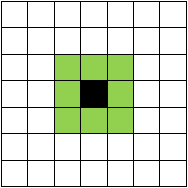
\includegraphics[width=3cm]{Nbhd_moore_1.png}
    \caption{Le voisinage de \bsc{Moore}, en vert}
    \label{fig:moore}
\end{figure}

\subsection{Mise en place du modèle, inspiré de \emph{Wa-Tor}}

\emph{Wa-Tor} est une simulation des interactions entre deux espèces sous forme d'automate cellulaire.  La simulation se déroule selon les règles suivantes:

\paragraph{Étape 1: Comportement des proies}
Chaque proie est dotée d'une variable interne qui croît à chaque génération jusqu'à ce qu'elle atteigne un "âge de reproduction". Son comportement est défini par cet ensemble de règles:
\begin{enumerate}
    \item La proie se déplace aléatoirement vers une case libre située dans son voisinage de Moore.
    \item Si elle a atteint son âge de reproduction, elle laisse derrière elle une nouvelle proie et sa variable interne est réinitialisée à $0$, comme celle de son nouveau-né.
    \item Sinon, son compteur interne est incrémenté de $1$.
\end{enumerate}
On remarque que les proies ne meurent alors jamais. On peut justifier cela par le fait que l'incapacité à mourir d'une proie équivaut en quelque sorte à ce qu'elle ait donné naissance à deux fils au lieu d'un lors d'une étape de la simulation.

\paragraph{Étape 2: Comportement des prédateurs}
Le comportement des prédateurs est plus complexe. Ils sont dotés de deux variables internes: leur âge de reproduction, comme pour les proies, ainsi que leur âge de "famine" \ie l'âge auquel ils meurent s'ils n'ont trouvé aucune proie à manger jusque là. Les règles deviennent alors:
\begin{enumerate}
    \item S'il a atteint son âge de famine, le prédateur meurt.
    \item Sinon, s'il détecte une ou plusieurs proie(s) dans son voisinage, il se déplace et prend la place d'une des proies au hasard. S'il a de plus atteint l'âge de reproduction, il laisse derrière lui un nouveau prédateur, d'âge de famine identique et d'âge de reproduction $0$.
    \item On augmente le compteur de famine de $1$ s'il n'y a pas de proie, et celui de reproduction aussi s'il n'a pas donné naissance à un nouveau-né.
\end{enumerate}

J'ai repris cet algorithme en y apportant quelques modifications. Déjà l'ajout d'une variable $\beta$, de même nom que le paramètre du système $(LK)$ car son rôle est similaire. Les prédateurs ont ainsi une probabilité $\beta$ d'attraper une des proies dans son voisinage. De plus, les cellules de la grille peuvent prendre un quatrième état, celui d'"obstacle", pour rendre compte de l'effet du milieu sur l'interaction entre proies et prédateurs. Ces cases obstacles restent dans le même état tout au long de la simulation.

\subsection{Description générale du programme}

J'ai choisi le langage Python pour développer mon modèle. La simulation se présente sous la forme d'une interface graphique dans laquelle l'utilisateur peut choisir lui même la répartition et les paramètres relatifs aux deux espèces. J'ai utilisé le module graphique intégré dans Python \textsf{tkinter}, qui n'est pas la plus optimisée des interfaces mais qui reste adaptée à mon projet. D'autres modules m'ont été nécessaire, notamment \textsf{numpy} pour optimiser légèrement les opérations itératives sur les listes de grande taille, \textsf{random} pour la gestion de l'aléatoire et \textsf{matplotlib.pyplot} pour la création et l'affichage de graphiques.

\paragraph{La programmation orientée objet}
J'ai développé mon programme en programmation orienté objet. La programmation objet possède de nombreux atouts, dont celui de structurer le script en l'organisant comme un ensemble de méthodes qui interagissent entre elles et avec d'autres programmes. Elle introduit le concept d'encapsulation: les variables et les méthodes utilisées sont "enfermées" dans l'objet, ce qui facilite l'exportation du script dans d'autres programmes. Une conséquence importante de ceci est la disparition quasi-totale des variables globales, et donc de sources d'erreurs potentielles. Enfin, la programmation objet offre la possibilité de construire de nouveaux objets à partir d’objets préexistants sans les modifier: c'est le concept de \emph{dérivation}. La classe principale de mon programme, appelée \textsf{ProiePredateur}, est ainsi construite par dérivation de la classe des cadres \textsf{Frame} de \textsf{tkinter}.

\paragraph{L'espace de simulation}
La fenêtre principale est découpée en trois zones. D'abord le canevas, où se déroule la simulation. C'est une grille finie, constituée de $45 \times 55$ cellules de $12$ pixels de côté. La grille est de forme torique: les bords opposés se rejoignent deux à deux. En dessous de la grille, on trouve l'espace de gestion avec la génération et les populations de proie et de prédateur actuelles et les boutons de contrôle. Enfin à droite se situe l'espace des options avec le choix des paramètres relatifs aux espèces, la vitesse, l'affichage des graphes etc. La fenêtre principale est représentée figure \ref{fig:programme}.

Pour décrire l'état de la grille, on utilise de plus $5$ tableaux à deux dimensions: \textsf{t[x, y]} désigne alors la case de la grille en $(x, y)$:
\begin{itemize}[label=\textbullet]
    \item \textsf{grille\_vie} qui attribut un des états suivants à chaque cellule de la grille: $0$ si la case est vide, $-1$ si la case est un obstacle, $1$ si la case est occupée par une proie ou un prédateur. Ce tableau est utile lors de la détermination des cases obstacles et des voisins d'un individu;
    \item \textsf{grille\_proie} qui repère les proies et leur attache leur compteur de reproduction (à la création d'une proie, une valeur aléatoire entre $1$ et l'âge de reproduction des proies est attribuée à ce compteur pour éviter que toutes les proies ne donnent simultanément naissance à une nouvelle proie);
    \item \textsf{grille\_predat}, pareil que précédemment pour les prédateurs;
    \item \textsf{grille\_predatfaim} qui renseigne sur la faim de chaque prédateur. J'ai préféré séparer ce tableau du précédent à cause de la difficulté de créer et de gérer des tableaux de tuples avec \textsf{numpy};
    \item \textsf{grille\_items} qui contient les cellules en elles-mêmes. C'est grâce à ce tableau qu'on peut personnaliser chaque case de la grille. Cette liste permet de ne modifier que la couleur des cellules en fonction de la présence d'une espèce ou non plutôt que de créer de nouvelles cases à chaque itération.
\end{itemize}

\paragraph{L'algorithme}
Un clic est repère sur la grille par ses coordonnées (en pixels, qu'on convertit ensuite en position de cellule). On change alors la couleur de la case correspondante si une proie, un prédateur ou un obstacle est créé ou si l'on veut rendre la case vide. Au lancement de la simulation:
\begin{enumerate}
    \item On parcourt d'abord la liste des proies (\textsf{grille\_proie}). Pour chaque proie, on détermine les cases vides adjacentes en tenant compte de la forme torique de la grille et des obstacles, puis on applique l'algorithme vu précédemment (\emph{Étape $1$} de \emph{Wa-Tor}) en actualisant sa variable de reproduction (\ie \textsf{grille\_proie}) si nécessaire. La proie se déplace ensuite aléatoirement vers une case voisine libre.
    \item On parcourt ensuite la liste des prédateurs (\textsf{grille\_predat}). La fonction qui détermine son voisinage renvoie un tuple de liste: les cases vides voisines et les proies voisines. Si la première liste n'est pas vide, le prédateur mange une des proies (avec une probabilité $\beta$). Sinon, comme pour la proie, le prédateur se déplace aléatoirement et on actualise ses deux variables internes (\ie \textsf{grille\_predat} et \textsf{grille\_predatfaim}).
    \item On actualise la population de proies et de prédateurs et on actualise aussi la liste des effectifs utilisée qu'on utilisera pour afficher le graphe d'évolution.
    \item A la fin de cette itération, on rappelle la même méthode après une durée \textsf{v}, en $\si{\milli \second}$ déterminée par l'utilisateur.
\end{enumerate}
On remarque que l'ordre dans lequel on effectue l'étape $1$ et $2$ n'est pas insignifiant. J'ai choisi de commencer par les proies car il me semblait plus logique que les proies se déplacent les premières avant de se faire rattraper par les prédateurs.

\begin{figure}[!ht]
    \centering
    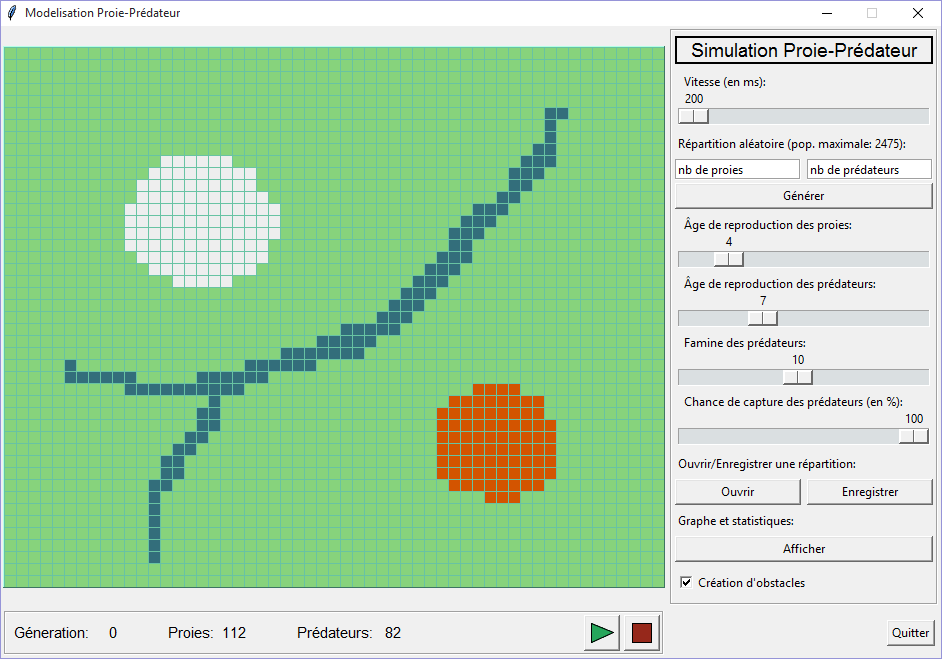
\includegraphics[width=15cm]{apercu_programme.png}
    \caption{Le programme final, dans une configuration initiale}
    \label{fig:programme}
\end{figure}

\subsection{Commentaires sur l'algorithme}

\paragraph{Complexité}
La complexité spatiale est en $\grandO{T + N}$ où $T$ est le nombre de cellules de la grille et $N$ est le nombre de générations simulées, à cause des $5$ tableaux de taille $T$ et du tableau des effectifs de taille $N$.

Il est difficile d'évaluer précisément la complexité temporelle globale du programme à cause des nombreuses fonctions externes employées et du fait de la nature fondamentalement aléatoire des automates cellulaires et de l'évolution d'une population. On peut néanmoins estimer la complexité temporelle théorique du passage d'une génération à la suivante, en considérant que les opérations de lecture et de modification sur les listes ont un coût constant, de même pour les modifications visuelles (changement de couleur d'une case et actualisation de population). On suppose de plus que les fonctions \textsf{randint} et \textsf{choice} ont un coût linéaire par rapport à la taille des bornes et la liste passées en argument, soit un coût en $\grandO{100}$ et $\grandO{8}$ respectivement dans le programme. Alors si $p_1$ est le nombre de proies et $p_2$ le nombre de prédateurs, la complexité est en $\grandO{p_1 + p_2}$.


Dans la pratique, on observe de légers ralentissements une fois la grille presque totalement remplie.

\paragraph{Analogies avec le système $(LK)$}
Les limites de ce modèle sont les mêmes que celles exposées pour le modèle de \emph{Lotka-Volterra}, exceptées le fait qu'il soit possible ici de créer artificiellement des contraintes environnementales par la placement d'obstacles.


Les paramètres relatifs aux espèces des deux modèles sont reliés par les relations suivantes:
\begin{itemize}[label=\textendash]
    \item L'âge de reproduction des proies correspond à $\frac{1}{\alpha}$.
    \item La probabilité qu'ont les prédateurs de capturer leur proie correspond à $\beta$.
    \item L'âge de famine des prédateurs correspond à $\frac{1}{\gamma}$.
    \item L'âge de reproduction des prédateurs correspond à $\frac{1}{\delta}$.
\end{itemize}
Dans la suite, $\alpha$, $\beta$, $\gamma$ et $\delta$ correspondront aux paramètres de la simulation et non plus à ceux du modèle théorique.

\section{Résultats et comparaison des modèles}

On emploie la bibliothèque \textsf{matplotlib.pyplot} pour afficher un graphique à n'importe quel moment de la simulation. Grâce au tableau des populations actualisée à chaque itération, on peut ainsi tracer le nombre de proies et de prédateurs en fonction de la génération. Cette option nous permet de comparer notre modèle au système $(LK)$ et à l'évolution réelle évoquée au début.

\subsection{Stabilité du système}
Avec les paramètres par défaut, sur une grille sans obstacles, on peut observer une évolution stable et périodique des populations, qui se traduit par un phénomène migratoire des proies chassées par les prédateurs dans une direction donnée (figure \ref{fig:stable}). La population des proies croît, faisant alors proliférer les prédateurs. Mais un surplus de prédateur entraîne alors une diminution du nombre de proie, ce qui à son tour fait baisser les effectifs des prédateurs, et le cycle recommence.

\begin{figure}[!ht]
    \begin{subfigure}{0.49\textwidth}
        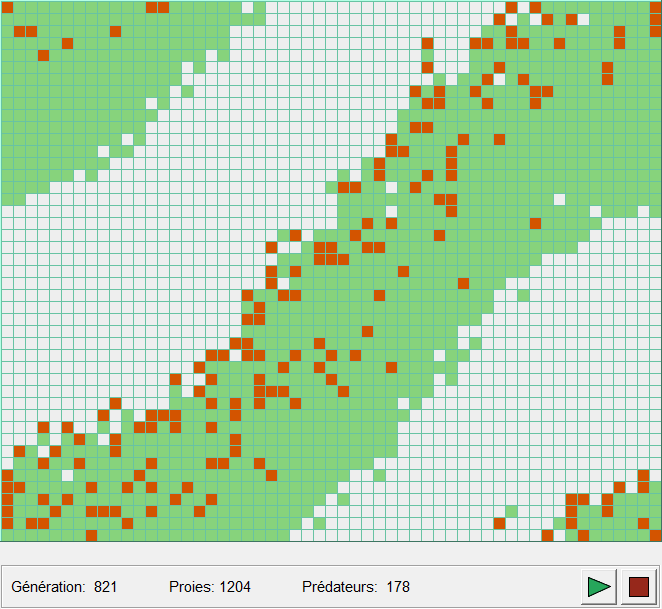
\includegraphics[width=\linewidth]{phenomene_migratoire2.png} 
        \caption{Le phénomène migratoire}
    \end{subfigure}
    \begin{subfigure}{0.49\textwidth}
        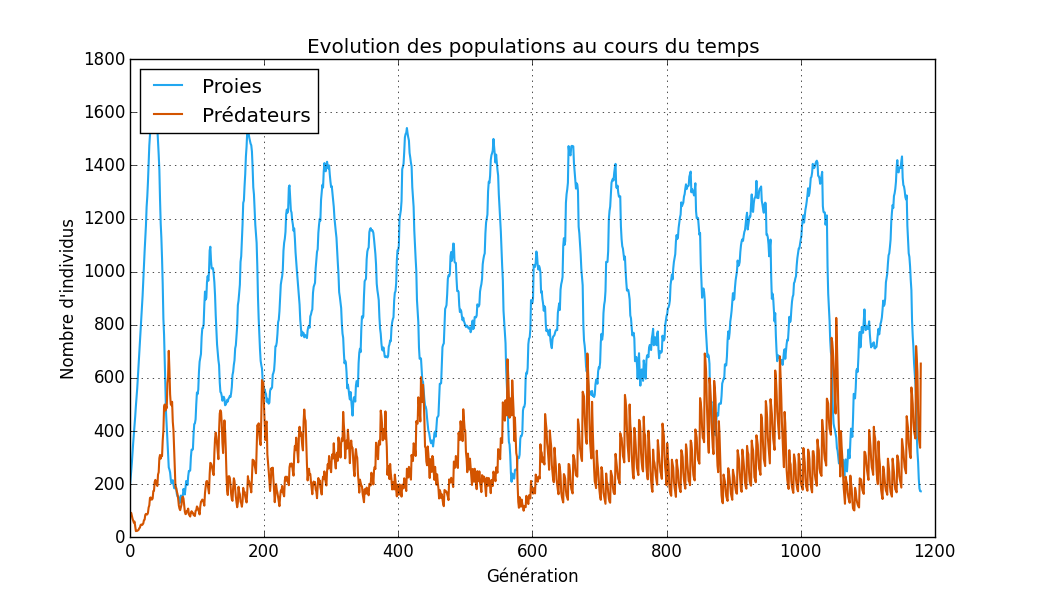
\includegraphics[width=\linewidth]{graphe_config_stable.png}
        \caption{Le graphe obtenu}
    \end{subfigure}
     
    \caption{Une configuration stable}
    \label{fig:stable}
\end{figure}

\subsection{Influence des options}
En l'absence de prédateurs, on remarque déjà la croissance exponentielle des proies, jusqu'à ce que la population remplisse tout l'espace. En l'absence de proie, les prédateurs s'éteignent en l'espace de quelques générations.


\paragraph{Influence de la position initiale et du milieu}
Pour évaluer l'influence spatiale sur la simulation, on fixe déjà les paramètres des espèces à leur valeur par défaut: $(\alpha = 4, \beta = 1, \gamma = 10, \delta = 7)$.
Une répartition trop aléatoire des deux espèces entraîne dans la grande majorité des cas l'extinction des proies, puis celle des prédateurs. En effet, dans ce cas les proies n'ont pas le temps de proliférer et sont immédiatement capturées. On s'intéressera donc à des répartitions par troupeaux.

On observe ainsi deux phénomènes prévisibles: lorsque les prédateurs sont à une distance des proies supérieure au nombre de générations qu'ils sont capables de supporter sans nourriture (\ie leur âge de famine), ils finissent par mourir. De même, un obstacle entre les deux troupeaux entraîne la disparition des prédateurs.

Enfin, si on place des obstacles aléatoirement sur la grille, les deux populations interagissent plus longtemps que dans les cas précédents, mais les prédateurs l'emportent quand même sur les proies (figure \ref{fig:aleatoire}). On peut expliquer ce résultat par le fait que les proies se retrouvent à un moment piégées, sans possibilité de s'enfuir indéfiniment, et donc se font attraper.

\begin{figure}[!ht]
    \begin{subfigure}{0.49\textwidth}
        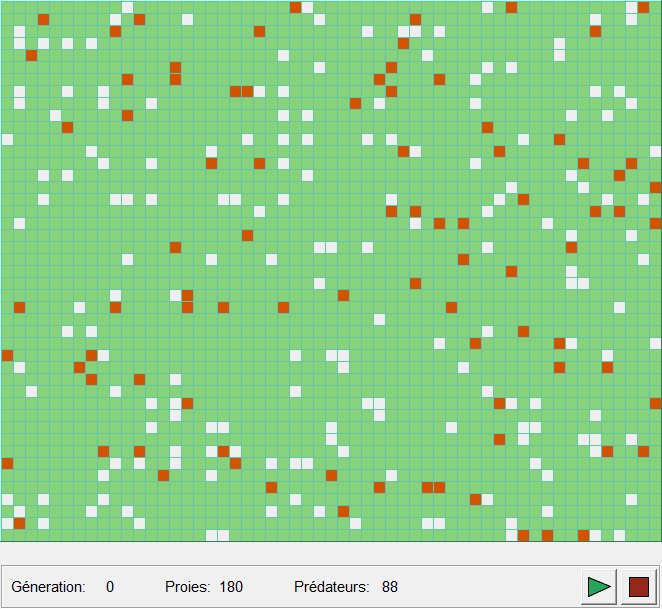
\includegraphics[width=\linewidth]{repart_aleatoire2.png} 
        \caption{Une répartition aléatoire initiale}
    \end{subfigure}
    \begin{subfigure}{0.49\textwidth}
        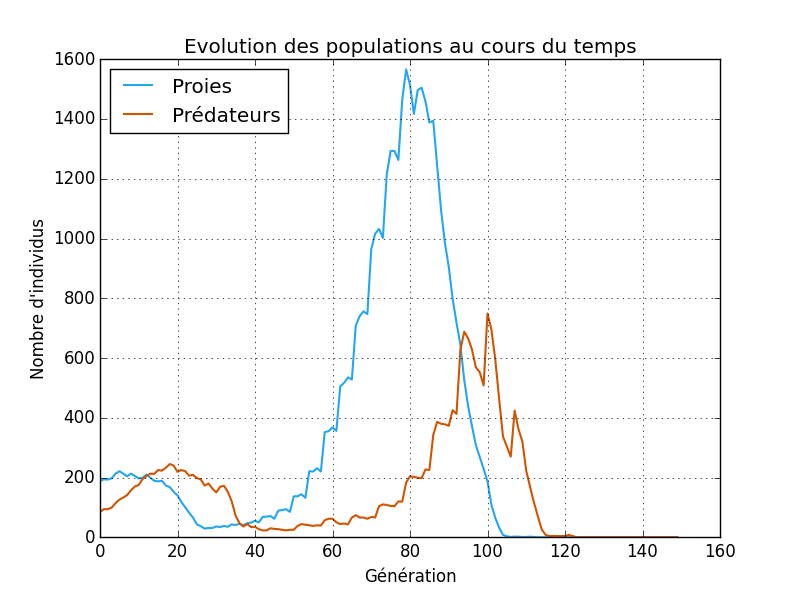
\includegraphics[width=\linewidth]{repart_aleat_resultat1.png}
        \caption{Le graphe obtenu}
    \end{subfigure}
     
    \caption{Résultat d'une répartition aléatoire}
    \label{fig:aleatoire}
\end{figure}


\paragraph{Influence des paramètres}
Pour évaluer l'influence des paramètres relatifs aux deux espèces, on considère la grille vide de tout obstacle, et on fixe les paramètres à leurs valeurs par défaut $(\alpha = 4, \beta = 1, \gamma = 10, \delta = 7)$ ainsi qu'une configuration initiale identique à chaque essai (telle que les prédateurs aient au moins une chance d'atteindre le troupeau de proies).

\subparagraph{Variation de $\alpha$, l'âge de reproduction des proies:}

Comme on peut s'y attendre, une faible valeur de $\alpha$ ($\leq 2$) conduit à une prolifération rapide des proies qui occupent finalement tout l'espace disponible en quelques générations. On observe deux type de résultat: les prédateurs ayant toujours de la nourriture à portée se développent tout aussi rapidement et dévorent toutes les proies avant de s'éteindre à leur tour, ou alors une configuration stable s'établit lorsque pour chaque proie tuée, une proie naît à la génération suivante.

Mais contre-intuitivement, une valeur de $\alpha$ élevée ($\geq 15)$ a pour conséquence la victoire quasi-permanente des proies sur les prédateurs, dont la population reste peu élevée au cours de la simulation. En effet, la reproduction très lente des proies rend la chasse du prédateur beaucoup moins fructueuse et l'espèce finit par s'éteindre après un grand nombre de générations (figure \ref{fig:taux_proie_eleve}).

\begin{figure}[!ht]
    \centering
    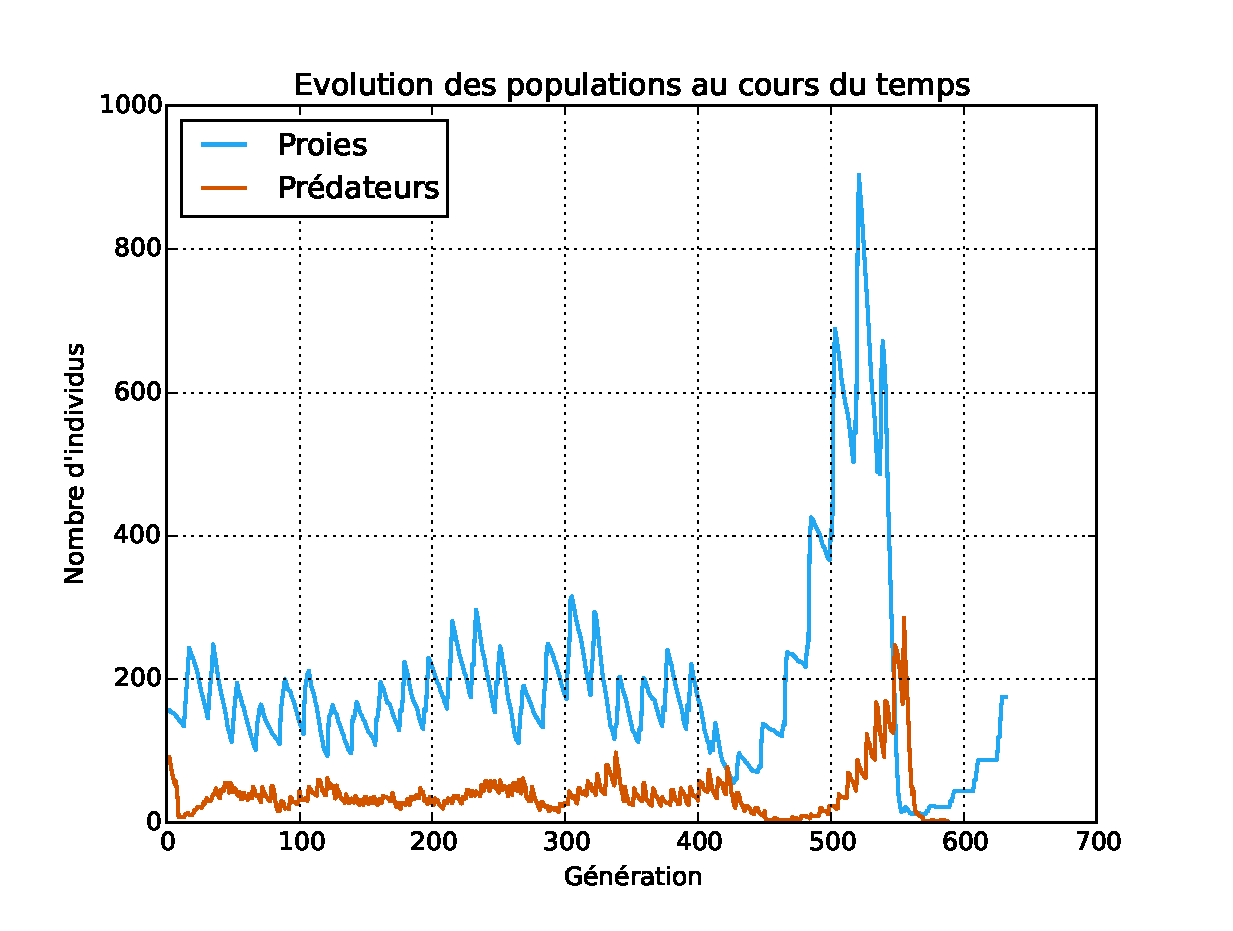
\includegraphics[width=12cm]{taux_proie_grand.eps}
    \caption{Évolution pour $\alpha = 18$: disparition des prédateurs à la génération $588$}
    \label{fig:taux_proie_eleve}
\end{figure}

\subparagraph{Variation de $\beta$, la probabilité de capture d'une proie par un prédateur:}

Pour des valeurs médianes de $\beta$ ($0.15 \leq \beta \leq 0.85$), l'influence de ce paramètre se ressent surtout sur la période des fluctuations de populations qui augmentent lorsque $\beta$ diminue. Il se présente de plus une tendance des prédateurs à migrer beaucoup plus lentement, puisqu'ils ont des proies toujours à proximité.

Pour de faibles valeurs de $\beta$ ($\beta \leq 0.20$), les effets précédents s'accentuent. En plus de cela, après un certain temps, on observe une homogénéisation des deux populations: la grille est alors occupée par les deux espèces en nombre à peu près égal pour le reste de la simulation (figure \ref{fig:faible_proba}).
Les individus se mélangent du fait de la difficulté des prédateurs à chasser efficacement, et donc de faire fuir le troupeau des proies.

\begin{figure}[!ht]
    \centering
    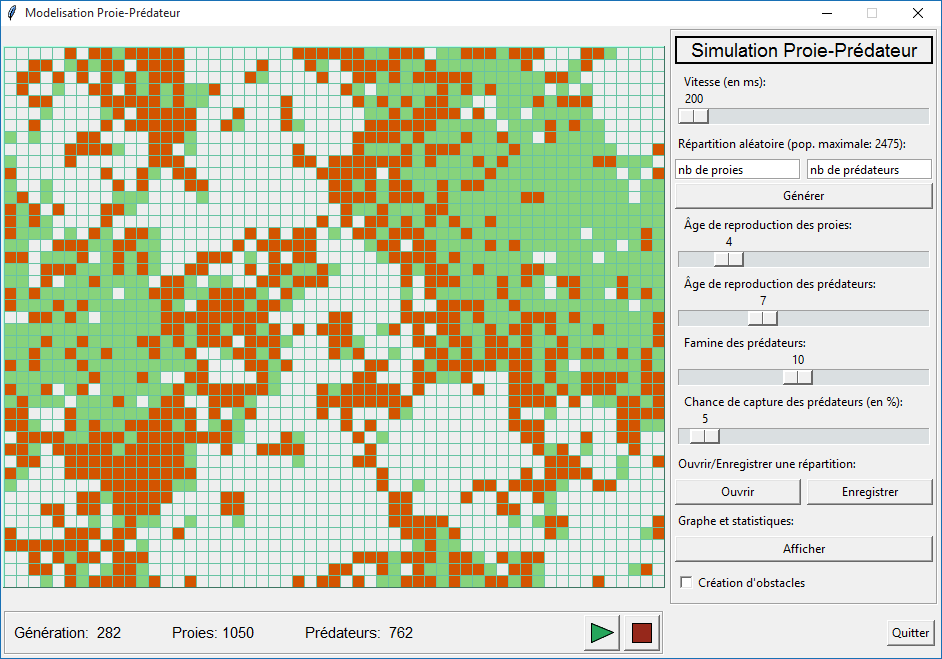
\includegraphics[width=12cm]{faible_proba.png}
    \caption{Un exemple d'évolution pour une probabilité $\beta = 0.05$}
    \label{fig:faible_proba}
\end{figure}


\subparagraph{Variation de $\gamma$, le délai avant lequel les prédateurs meurent de faim:}

Sans grande surprise, une valeur élevée de $\gamma$ conduit toujours à la victoire des prédateurs après un nombre plus ou moins grand d'itérations. Inversement, une valeur faible du paramètre mène à l'extinction des prédateurs, qui ne sont plus capables de capturer des proies à moins qu'elles ne soient dans leur voisinage immédiat.

\subparagraph{Variation de $\delta$, l'âge de reproduction des prédateurs:} 

Une faible valeur de $\delta$ ($ \leq 5 $) mais supérieure à $\alpha$ rend les chances d'obtenir une évolution stable grandes car la naissance de nouveaux prédateurs réussit à compenser les pertes dues à la famine. Mais lorsque cette valeur est inférieure à $\alpha$, les prédateurs se reproduisent plus vite que les proies et donc progressivement prennent le dessus en terme de population sur ces dernières, jusqu'à l'extinction des proies.

Une grande valeur de $\delta$ ($ \geq 15 $) n'implique pas nécessairement la disparition des prédateurs. On observe surtout une évolution plus lente de leur population, qui peut leur être bénéfique car les proies ont dans ce cas le temps de se reproduire et de remplir l'espace. Les prédateurs restent alors en nombre réduit et ne manquent  jamais de nourriture, ce qui est propice à l'apparition d'un système stable (figure \ref{fig:taux_predat_eleve}).

\begin{figure}[!ht]
    \centering
    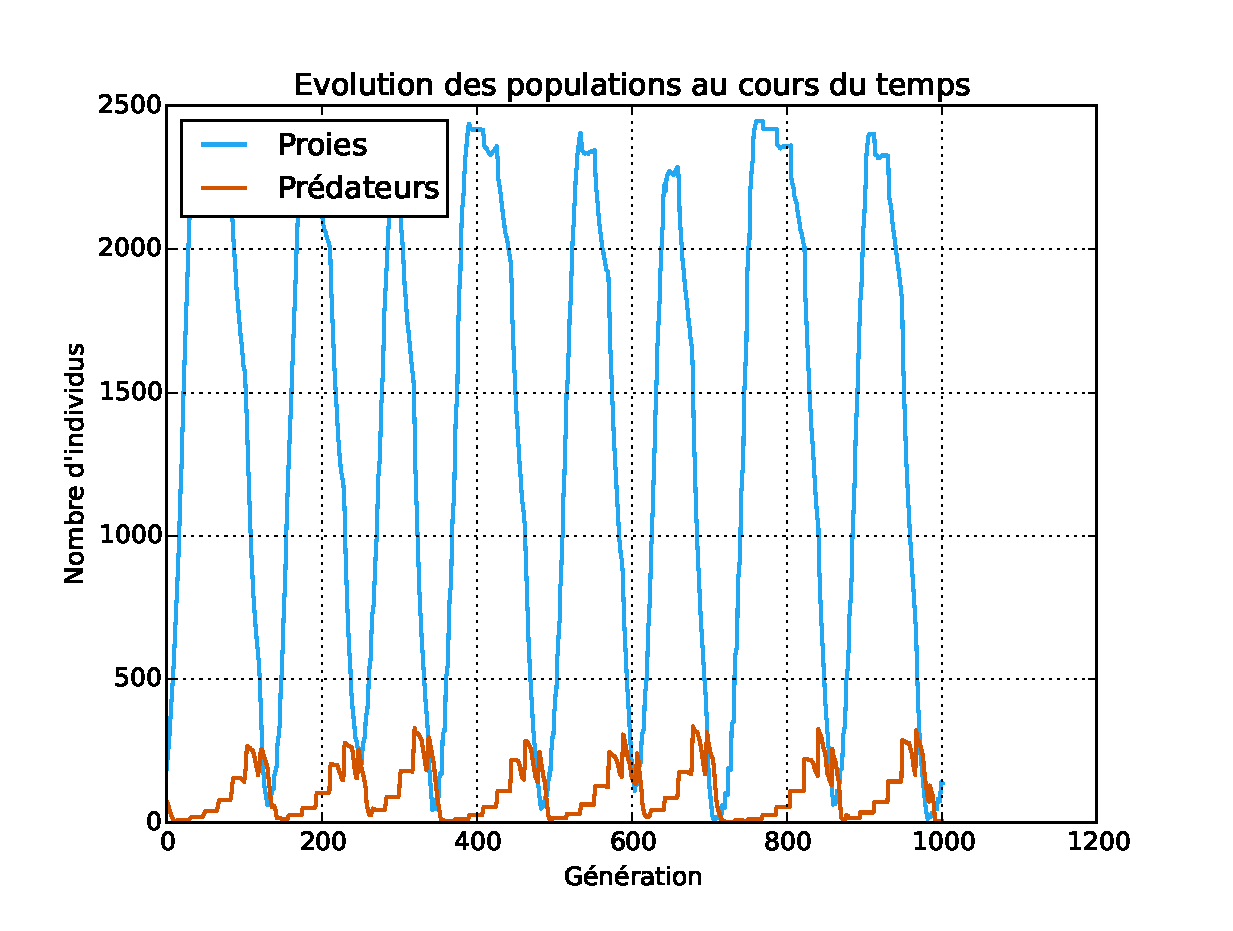
\includegraphics[width=12cm]{taux_predat_grand.eps}
    \caption{Évolution pour $\delta = 18$ aboutissant à un système stable}
    \label{fig:taux_predat_eleve}
\end{figure}


\subsection{Comparaison aux modèles théoriques et réels}

On remarque déjà la similarité des graphiques obtenues lors du suivi des populations entre celui théorique de $(LK)$, celui réel (figure \ref{fig:baie_hudson}) et celui de notre modèle en configuration stable (figure \ref{fig:stable}) qui se traduit par une évolution quasi-périodique des effectifs. Le modèle informatique, tout comme le modèle théorique, est par ailleurs sensible aux variations des paramètres propres aux espèces, ce qui rend possible diverses interprétations sur le rôle de chacune d'entre elles. De plus, la simulation et le modèle $(LK)$ ont les mêmes comportements en l'absence d'une des deux espèces.

On note toutefois l'aspect piqué du graphe de l'automate cellulaire. Cela s'explique par le choix de la discrétisation du temps qui fait qu'à partir d'un certain temps, les paramètres concernant les taux de reproduction et de famine se synchronisent entre les individus entraînant alors des petites augmentations ou diminutions brusques des populations. De même, la courbe d'une évolution réelle présente des discontinuités dues pareillement à l'étude non continue du processus mais aussi à des dizaines d'autres facteurs non pris en compte dans les modèles théoriques et informatiques (exposés en partie à la section \ref{limites}).

\section{Conclusion}

Nous avons vu ici comment il était possible d'implémenter un modèle théorique, les équations de \textsc{Lotka-Volterra}, à travers une simulation dynamique afin de mieux comprendre le rôle que peuvent jouer les divers paramètres. A l'aide de divers outils informatiques: automate cellulaire, programmation objet, interface graphique, analyse numérique, manipulation de matrices et de graphiques, j'ai pu traduire un processus complexe et d'apparence aléatoire sous forme d'interactions simples entre individus de différentes espèces. Cette modélisation a pour aspiration de se rapprocher le plus fidèlement possible d'un phénomène réel et continu, celui de la dynamique des populations, dont la compréhension est devenue de nos jours primordiale, tout en restant dans le cadre fixé par le thème des TIPE de cette année.

\newpage
\section{Annexe}\label{annexe}

\paragraph{Bibliothèques importées et création de la classe \textsf{ProiePredateur}}
Au lancement du programme, on définit une nouvelle classe dérivant de la classe \textsf{Frame} de \textsf{tkinter} et on initialise les constantes.

\begin{minted}[frame=lines, linenos]{python}

from tkinter import *
from random import randint, choice
from time import clock
import matplotlib.pyplot as plt
import numpy as np
import pickle #Permet d’enregistrer des données avec conservation de leur type
#Module donnant accès aux fenêtres de recherche de fichiers:
from tkinter.filedialog import asksaveasfile, askopenfile


class ProiePredateur(Frame):
    """La classe principale de la simulation proie prédateur et ses méthodes."""
    def __init__(self, master):
        Frame.__init__(self, master)

        self.width       = 660                 #Largeur du canevas
        self.height      = 540                 #Hauteur du canevas
        self.xmax = self.width  // 12          #Nombre de case en largeur
        self.ymax = self.height // 12          #Nombre de case en hauteur 
        #Vitesse par defaut de la simulation, en ms:
        self.vitesse     = 200                     
        self.coul_fond   = "#87D37C"           #Couleur du fond
        #Couleur des proies/prédateurs respectivement:
        self.coul_cel    = ["#EEEEEE", "#D35400"] 
        #Couleur des lignes de séparation  
        self.coul_lignes = "#68C3A3"                
        self.coul_milieu = "#336E7B"           #Couleur des obstacles
        #Variable de contrôle: simulation active (=1) ou non:
        self.flag = 0                               
        self.proie_cfg = 4                     #Age de reproduction des proies
        #Age de reprod/Age de famine des prédateurs respectivement:
        self.predat_cfg = [7, 10]    
        #Chance qu'a le prédateur de capturer sa proie:
        self.chance_capture = 100 

\end{minted}

\paragraph{Initialisation de la simulation:}
Cette méthode est appelée lors du lancement du programme et à chaque fois que l'utilisateur clique sur le bouton stop.

\begin{minted}[frame=lines, linenos]{python}

def nouv_grille(self):
    "Affiche l'espace de simulation et initialise les variables."
    #Permet d'éviter une itération en trop lorsqu'une simulation est en cours
    if self.flag:                                   
        self.flag = 0
        self.after(self.vitesse, self.nouv_grille)  
        return
        
    self.change_bouton(1)       #Affichage du bouton Play
    self.can.delete(ALL)        #Efface le canevas
        
    #Initialisation des variables:
    
    self.generation = 0         #Compteur de génération
    #Tableau contenant respectivement le nombre de proies et 
    #le nombre de prédateurs actuel:
    self.pop = [0, 0]       
    
    #Tableau contenant les populations à chaque génération
    #(cet historique est utile lors du tracé de graphes)
    self.evol_pop =([], []) 
    
    #Tableau des proies contenant pour chaque coordonnées
    #l'âge de la proie (> 0 ou 0 si pas de proie):
    self.grille_proie = np.zeros( (self.xmax, self.ymax), dtype = np.int8)
    #Pareil pour les prédateurs:
    self.grille_predat = np.zeros( (self.xmax, self.ymax), dtype = np.int8)
    #Tableau contenant la 'faim' actuelle du prédateur
    self.grille_predatfaim = np.zeros( (self.xmax, self.ymax), dtype = np.int8)   
    #Tableau repérant les cases vivantes, d'obstacles et vides (-1):
    self.grille_vie = np.zeros( (self.xmax, self.ymax), dtype = np.int8)
    #Tableau contenant les cases en elles-mêmes:
    self.grille_items = np.empty( (self.xmax, self.ymax), dtype = np.object) 
    
    #Créer les cellules et les place dans grille_items
    for x in range(self.xmax): 
        for y in range(self.ymax): 
            self.grille_items[x, y] = self.can.create_rectangle(x*12+3, y*12+3,
            x*12+15, y*12+15, fill=self.coul_fond, outline=self.coul_lignes)
    
    #On initialise l'affiche de la génération et des populations
    self.showgen.config(text="Géneration: {:5}".format(0))
    self.showproie.config(text="Proies: {:4}".format(0))
    self.showpredat.config(text="Prédateurs: {:4}".format(0))

\end{minted}

\paragraph{Coordonnées des cellules voisines}
Cette méthode permet de récupérer les cellules voisines vides d'une proie ou d'un prédateur. Ici, ce sont les cellules voisines vides d'une proie qu'on récupère. Le principe est le même pour un prédateur, mais il faut cette fois examiner en plus les cellules voisines contenant des proies.

\begin{minted}[frame=lines, linenos]{python}

def cel_voisines_proie(self, x, y):
    "Retourne un tableau contenant les coord des cellules vides voisines\
     de la proie en (x, y)."
    v = []
    for i in range(-1, 2, 1):
        for j in range(-1, 2, 1):
            #L'opération modulo permet de considérer la grille comme torique:
            x2, y2 = (x + j)%self.xmax, (y + i)%self.ymax      
            if not self.grille_vie[x2, y2]: v.append((x2, y2))
                
\end{minted}

\paragraph{Lancement de la simulation}
Cette méthode récursive effectue les tests nécessaires à la détermination de la prochaine génération pour finalement s'appeler elle-même après un délai fixé par l'utilisateur.

\begin{minted}[frame=lines, linenos]{python}

def animation(self):
    "Simule l'évolution des populations, en tenant compte des paramètres."
    t1 = clock()
    
    #On commence par parcourir les cases contenant les proies
    for x, y in np.transpose(np.nonzero(self.grille_proie)):    
        #Récupère les cases vides adjacentes:
        v = self.cel_voisines_proie(x, y)   
        if v != []:
            reprod = self.grille_proie[x, y]
            #La proie choisit une case au hasard vers laquelle se déplacer:
            x2, y2 = choice(v)  
            if reprod >= self.proie_cfg: #Naissance d'une nouvelle proie
                #'proie_vie' fait apparaître une proie aux coord fournies:
                self.proie_vie(x2, y2, 1) 
                self.grille_proie[x, y] = 1
            else: 
                #Déplace la proie et incrémente sa variable interne:
                self.proie_vie(x2, y2, reprod+1) 
                self.tue_cellule(x, y, 1)
        else: self.grille_proie[x, y] += 1
    
    #Puis on parcout les cases contenant les prédateurs
    for x, y in np.transpose(np.nonzero(self.grille_predat)):
        #v est un tuple de tableaux renvoyé 'par cel_voisines_predat':
        v = self.cel_voisines_predat(x, y) 
        faim = self.grille_predatfaim[x, y]
        #Si le prédateur est affamé, on le tue:
        if faim >= self.predat_cfg[1]: self.tue_cellule(x, y, 2)    
        elif v != ([], []):
            reprod = self.grille_predat[x, y]
            #Si il y a une proie à coté, et que le prédateur 
            #réussit à l'attraper, il prendra sa place:
            if v[1] != [] and (randint(1, 100) <= self.chance_capture\
                or v[0] == []): 
                x2, y2 = choice(v[1])
                self.tue_cellule(x2, y2, 1)
                faim = 0
            else: x2, y2 = choice(v[0]) #Sinon, déplacement vers une case vide:
            #Le prédateur peut donner naissance à une nouvelle proie:
            if reprod >= self.predat_cfg[0]: 
                self.predat_vie(x2, y2, 1, faim + 1)
                self.grille_predat[x, y] = 1
                self.grille_predatfaim[x, y] = faim + 1
            else: #Déplace le prédateur
                self.predat_vie(x2, y2, reprod+1, faim+1)
                self.tue_cellule(x, y, 2)
        else: 
            self.grille_predat[x, y] += 1
            self.grille_predatfaim[x, y] += 1
    
    #La génération est incrementée de 1, puis on actualise l'affichage
    self.generation += 1    
    self.showgen.config(text="Génération: {:4}".format(self.generation))
    #On ajoute les effectifs dans le tableau des relevés:
    self.evol_pop[0].append(self.pop[0])  
    self.evol_pop[1].append(self.pop[1])
    
    #Rappelle la fonction d'animation après un certain temps 'vitesse' (en ms)
    if self.flag:        
        t = int((clock()-t1)*1000)
        #On tient ici compte du délai provenant des tests précédents:
        if t < self.vitesse: self.after(self.vitesse - t, self.animation)   
        else: self.after(0, self.animation)

\end{minted}

\paragraph{Affichage des graphiques}
Cette méthode utilise la bibliothèque \textsf{matplotlib.pyplot} pour tracer le graphe des populations au cours du temps.

\begin{minted}[frame=lines, linenos]{python}
        
def affiche_graphes(self):
    "Trace le graphe de l'évolution des populations au cours de la simulation."
    if self.flag:   
        self.pause()
        self.after(self.vitesse, self.affiche_graphes)
        return
        
    gen = range(self.generation)
    plt.title("Evolution des populations au cours du temps")
    plt.plot(gen, self.evol_pop[0], linewidth=1.5, 
        color="#22A7F0", label="Proies")
    plt.plot(gen, self.evol_pop[1], linewidth=1.5, 
        color="#D35400", label="Prédateurs")
    plt.legend(loc='upper left')
    plt.xlabel("Génération")
    plt.ylabel("Nombre d'individus")
    plt.grid()
    plt.show()
    
\end{minted}

\paragraph{Affichage des solutions du système $(LK)$}
Grâce à la bibliothèque \textsf{matplotlib.pyplot} et la bibliothèque \textsf{scipy.integrate}, on peut tracer les graphes des solutions et le champ de vecteurs associé du système $(LK)$.

\begin{minted}[frame=lines, linenos]{python}

import matplotlib.pyplot as plt
import scipy.integrate as itg
import numpy as np

def LK(y, t):       #Les équations de Lotka-Volterra
    return np.array([ a*y[0]*y[1] - b*y[0], -c*y[0]*y[1] + d*y[1] ])

a, b, c, d = 1, 4, 1, 6       #Les constantes relatives aux proies
y0 = np.array([1., 1.])       #Les populations initiales
t = np.linspace(0, 10, 1000) #1000 points entre t=0 et t=10, pas constant

#Tracé du graphe:

#odeint renvoie une matrice des valeurs approchées de la solution:
v = itg.odeint(LK, y0, t)    
plt.title("Allure de la solution pour (x0, y0) = (1, 1)\
    et (a, b, c ,d) = (1, 4, 1, 6)")
plt.plot(t, v[:, 0], linewidth=1.5, color="#22A7F0", label="Proies")
plt.plot(t, v[:, 1], linewidth=1.5, color="#D35400", label="Prédateurs")
plt.legend(loc='upper left')
plt.xlabel("Temps")
plt.ylabel("Nombre d'individus")
    
#Tracé du champ de vecteurs:

x = np.linspace(0, 10, 20)
y = np.linspace(0, 10, 20)
#'meshgrid' retourne la matrice des coordonnées d'après les vecteurs coordonnées
X1, Y1 = np.meshgrid(x, y)
DX1, DY1 = LK([X1, Y1], 0)
M = np.hypot(DX1, DY1)
DX1 /= M
DY1 /= M
plt.title("Champ de vecteurs associé")
plt.xlabel("x(t)")
plt.ylabel("y(t)")
#Pour une grille de points (xi, yi), 'quiver' calcule les vecteurs normalisés
#de même direction que LK(xi, yi):
plt.quiver(X1, Y1, DX1, DY1, M)

plt.grid()
plt.show()

\end{minted}

\end{document}
